%settings

\setlength{\parindent}{2ex}
\phantomsection
%text
%-Task1----------------------------------
\section{Model of the application using Component Diagrams}
\par
\begin{figure}[h!]
	\centering
	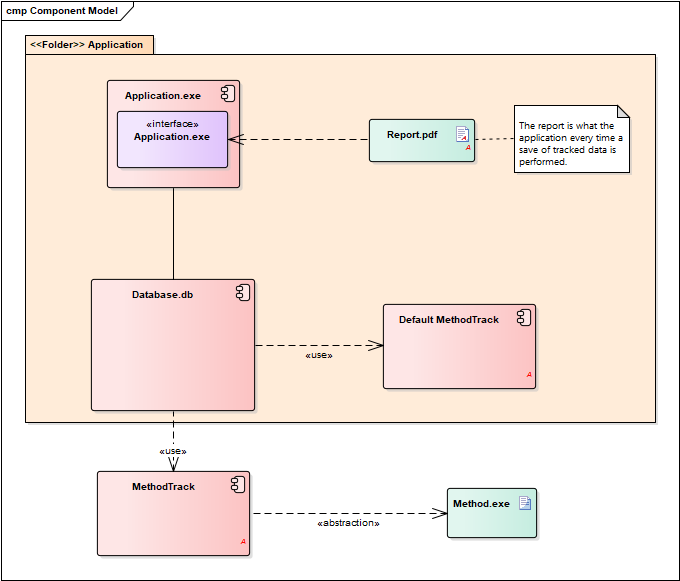
\includegraphics[width=\textwidth]{ComponentModel}
	\caption{Class Diagram} 
\end{figure}
The application executable in fig \thesection.1 is contained in its own specific folder and by running it we get the interface.
The database can use methods from outside the application folder and the default ones.
Each time a save is performed the the application generates a Report.pdf that outputs the tracked data in an easy way for the user to understand.
%-Task2----------------------------------
\newpage
\section{Steps needed to setup the project.}
In order to setup the project:
\begin{itemize}
\item[•] Download and install Qt(framework)
\item[•] Download and install Sql management studio.
\item[•] A team that is specialized in operating with data under windows,Mac os and Linux to create the default methods that the application is sought to provide by default.
\end{itemize}

\clearpage
